%----------------------------------------------------------------------------------------
%	PREÁMBULO
%----------------------------------------------------------------------------------------


\documentclass[11pt, oneside]{book}
\usepackage[paperwidth=17cm, paperheight=22.5cm, bottom=2.5cm, right=2.5cm]{geometry}

% El borde inferior puede parecerles muy amplio a la vista. Les recomiendo hacer una prueba de impresión antes para ajustarlo

\usepackage{amssymb,amsmath,amsthm} % Símbolos matemáticos
\usepackage[spanish,mexico,es-tabla]{babel}
\usepackage[utf8]{inputenc} % Acentos y otros símbolos 
\usepackage{enumerate}
\usepackage{optidef}
\usepackage{hyperref} % Hipervínculos en el índice
\usepackage[spanish]{cleveref}
\usepackage{graphicx}
\usepackage[usenames,dvipsnames]{xcolor} % Color
%\usepackage{subfig} % Subfiguras
\usepackage{listings}%Para los códigos de MALTAB, ver documentación de matlab-prettifier
\usepackage[framed]{matlab-prettifier}
\usepackage[linesnumbered,lined,boxruled,spanish,onelanguage]{algorithm2e}
\usepackage{titling}
\usepackage{amsfonts}
\usepackage[thinc]{esdiff}
\spanishdecimal{.}
\definecolor{itamgreen}{RGB}{0,104,83}
\hypersetup{
    colorlinks=true,
    linkcolor=itamgreen,
    filecolor=itamgreen,      
    urlcolor=itamgreen,
    citecolor=itamgreen
}
\urlstyle{same}


\usepackage{translations}
\graphicspath{{Imagenes/}} % En qué carpeta están las imágenes

\DeclareTranslationFallback{rank}{rank}
\DeclareTranslation{english}{rank}{rank}
\DeclareTranslation{spanish}{rank}{rango}

\DeclareMathOperator{\rank}{\GetTranslation{rank}}


% Para eliminar guiones y justificar texto
\tolerance=1
\emergencystretch=\maxdimen
\hyphenpenalty=10000
\hbadness=10000

\linespread{1.25} % Asemeja el interlineado 1.5 de Word

\let\oldfootnote\footnote % Deja espacio entre el número del pie de página y el inicio del texto
\renewcommand\footnote[1]{%
\oldfootnote{\hspace{0.05mm}#1}}

\newcommand{\bigO}[1]{\ensuremath{\mathop{}\mathopen{}\mathcal{O}\mathopen{}\left(#1\right)}}

\newcommand\smallO[1]{
    \mathchoice
    {% mode \displaystyle
      \scriptstyle\mathcal{O}\left(#1\right)
    }
    {% mode \textstyle
      \scriptstyle\mathcal{O}\left(#1\right)
    }
    {% mode \scriptstyle
      \scriptscriptstyle\mathcal{O}\left(#1\right)
    }
    {% mode \scriptscriptstyle
      \scalebox{0.7}{$\scriptscriptstyle\mathcal{O}$}\left(#1\right)
    }
}
  

\renewcommand{\thefootnote} {\textcolor{Black}{\arabic{footnote}}} % Súperindice a color negro

\setlength{\footnotesep}{0.75\baselineskip} % Espaciado entre notas al pie

\usepackage{fnpos} % Footnotes al final de pág.

\usepackage[justification=centering, font=bf, labelsep=period, skip=5pt]{caption} % Centrar captions de tablas y ponerlas en negritas

\newcommand{\imagesource}[1]{{\footnotesize Fuente: #1}}

\usepackage{tabularx} % Big tables
\usepackage{adjustbox}
\usepackage{longtable}


\usepackage{float} % Float tables

\usepackage{pgfplots} % Gráficas
\pgfplotsset{compat=newest}
\pgfplotsset{width=7.5cm}
\pgfkeys{/pgf/number format/1000 sep={}}

\newtheorem{theorem}{Teorema}[chapter]
\newtheorem{corollary}{Corolario}[theorem]
\newtheorem{lemma}[theorem]{Lema}
\newtheorem{definition}{Definición}
\newtheorem{plain}{Proposición}
\newtheorem{remark}{Corolario}[plain]

\newcommand{\Tr}[1]{\operatorname{Tr}\left(#1\right)}
\newcommand{\diag}[1]{\operatorname{diag}\left(#1\right)}
\newcommand{\frNm}[1]{\left\|#1\right\|_{\mathrm{F}}}

\SetKwBlock{Loop}{Repetir}{fin}

\usepackage{afterpage}
\newcommand\myemptypage{
    \null
    \thispagestyle{empty}
    \newpage
    }
    
    
\usepackage{todonotes}
%HAY Q BORRAR ESTOS COMMANDS EVENTUALMENTE
\newcommand{\val}[1]{\todo[color=blue!20!white]{\textbf{Vale:} #1}}
\newcommand{\valinline}[1]{\todo[inline,color=blue!20!white]{\textbf{Vale:} #1}}

\usepackage{natbib}

\usepackage{tcolorbox}

\usepackage{dirtytalk}

\usepackage[cache=false]{minted}
\usemintedstyle{bw}

\usepackage{multirow}

\begin{document}

%----------------------------------------------------------------------------------------
%	PORTADA
%----------------------------------------------------------------------------------------



\title{Una tesis extendida ($\overline{\text{tesis}}$)} 
\author{Valeria Aurora Pérez Chávez}

\begin{titlepage}
\begin{center}

\textsc{\Large Instituto Tecnológico Autónomo de México}\\[2em]

%Figura
\begin{figure}[h]
\begin{center}

\includegraphics[scale=0.9]{logo-ITAM.pdf}
\end{center}
\end{figure}

% Pueden modificar el tamaño del logo cambiando la escala

\textbf{\LARGE \thetitle}\\[2em]

\textsc{\large Tesis}\\[1em]

\textsc{\large que para obtener el título de}\\[1em]

\textsc{\LARGE Licenciado en Matemáticas Aplicadas}\\[1em]

\textsc{\large Presenta}\\[1em]

\textsc{\LARGE \theauthor}\\[1em]

\textsc{\large Asesor: Ernesto Juvenal Barrios Zamudio}\\[1em]


% Asegúrense de escribir el nombre completo de su asesor con grado académico

\end{center}

\vspace*{\fill}
\textsc{Ciudad de México \hspace*{\fill} 2021} %El otro año es el bueno

\end{titlepage}



%----------------------------------------------------------------------------------------
%	DECLARACIÓN
%----------------------------------------------------------------------------------------

\thispagestyle{empty}

\vspace*{\fill}
\begingroup

\noindent
«Con fundamento en los artículos 21 y 27 de la Ley Federal del Derecho de Autor y como titular de los derechos moral y patrimonial de la obra titulada ``\textbf{\thetitle}'', otorgo de manera gratuita y permanente al Instituto Tecnológico Autónomo de México y a la Biblioteca Raúl Bailléres Jr., la autorización para que fijen la obra en cualquier medio, incluido el electrónico, y la divulguen entre sus usuarios, profesores, estudiantes o terceras personas, sin que pueda percibir por tal divulgación una contraprestación.»


\centering 

\vspace{3em}

\textsc{\theauthor}

\vspace{5em}

\rule[1em]{20em}{0.5pt} % Línea para la fecha

\textsc{Fecha}
 
\vspace{8em}

\rule[1em]{20em}{0.5pt} % Línea para la firma

\textsc{Firma}

\endgroup
\vspace*{\fill}

\newpage


%----------------------------------------------------------------------------------------
%	DEDICATORIA
%----------------------------------------------------------------------------------------

\thispagestyle{empty}
\pagenumbering{gobble}

\chapter*{Agradecimientos}

Agradezco a facu por ser tan chingona y a Mike por pasarme el formato. Salu2.
\begin{flushright}
\textsc{El Serch}
\end{flushright}
\newpage


\pagestyle{plain}
\frontmatter
%----------------------------------------------------------------------------------------
%	RESUMEN
%----------------------------------------------------------------------------------------
\include{Chapters/Resumen}


%----------------------------------------------------------------------------------------
%	ÍNDICE GENERAL
%---------------------------------------------------------------------------------------

\tableofcontents %Opcional pero sugerido, en especial si como Paco van a escribir un libro de 500 páginas. Es tesis, no enciclopedia.

%----------------------------------------------------------------------------------------
%	ÍNDICE DE CUADROS Y FIGURAS
%---------------------------------------------------------------------------------------

\listofalgorithms %Opcional
\newpage

\listoftables %Opcional

\listoffigures %Opcional

%----------------------------------------------------------------------------------------
%	TESIS
%----------------------------------------------------------------------------------------

\mainmatter % Empieza la numeración de las páginas

\pagestyle{plain}

% Incluye los capítulos en el fólder de capítulos

\chapter{Introducción}

\say{I always promote \textsf{Julia} among friends and colleagues in Latin America, even when it has been difficult to convince them because of the scarce resources of \textsf{Julia} in Spanish. I firmly believe in open access knowledge without barriers (either language barriers, accessibility, or others), and I will always advocate for that} \cite{articulo_10anos}. Las palabras de la chilena Pamela Bustamente, usuaria de \textsf{Julia},  engloban la razón de ser de esta tesis. 

Mi camino con \textsf{Julia} comenzó a principios del 2021 cuando tuve la oportunidad de trabajar en el Instituto Mexicano del Seguro Social (IMSS). \textsf{Julia} fue la herramienta que utilice para desarrollar un proyecto que estaba fundamentado en estadística bayesiana y requería de una gran cantidad de simulaciones. No tarde mucho tiempo en encontrarme con las dificultades que menciona Pamela y algunas más. Sin embargo, \textsf{Julia} debe tener otras cualidades que frecuentemente lo destaquen como un lenguaje prometedor que cada día va tomando más fuerza en la comunidad de programadores. 

Al principio, dichas cualidades eran un misterio para mí. Mi interrogante principal fue sobre la necesidad de crear este nuevo lenguaje. ¿Por qué usar \textsf{Julia} y no \textsf{Python} o \textsf{R}?, ¿Cuál fue la motivación de su creación? y, después de encontrarme con una falta de recursos, ¿Cómo es posible que 10 años más tarde hay tan poca ayuda de este lenguaje?  Esta tesis es mi esfuerzo por mostrar un nuevo lenguaje, sus alcances y hacer una comparativa con lo que ya se conoce. De paso, mi trabajo queda como evidencia y punto de partida para futuros usuarios hispanohablantes.  

Este trabajo no es un manual de \textsf{Julia} ni de ningún otro lenguaje. Eso ya existe. Lo que se busca es explicar pros y contras que se encontraron al utilizar \textsf{Julia}, \textsf{Python} y \textsf{R} en tres ejercicios distintos.

La tesis se divide en dos partes. El propósito de la primera parte es dar una imagen general de las funciones que se utilizaron en los tres lenguajes para crear la segunda parte. Primero, se expone la instalación de \textsf{Julia} en un sistema operativo \textsf{Windows} para después explicar aspectos básicos del lenguaje. También, se da una introducción a dos paquetes fundamentales para este trabajo. Esto se hace pensando que \textsf{Julia} es el lenguaje más reciente y se busca que el lector navegue fácilmente por el código presentado. Después, se presentan los paquetes y funciones que se utilizaron en \textsf{Python} y en \textsf{R} suponiendo que el lector ya está familiarizado con ellos. 

La segunda parte de la tesis consta de tres ejercicios cuyo objetivo es mostrar un aspecto diferente en los lenguajes. El primer ejercicio toma datos del National Institute of Standards and Technology (NIST) para medir la precisión numérica de cada lenguaje al hacer el ajuste de un polinomio de grado 10. El segundo ejercicio usa los datos del Censo de Población y Vivienda de México del 2020 hecho por el Instituto Nacional de Estadística y Geografía (INEGI). El objetivo de este ejercicio es el manejo y manipulación de una gran cantidad de datos. Finalmente, el tercer ejercicio presenta la programación de un algoritmo de búsqueda que se utiliza en la discriminación de modelos en diseños de experimentos. En este ejercicio, los cálculos son más intensivos por lo que busca medir la capacidad y velocidad de cómputo de los lenguajes. 

A continuación, se comienza este trabajo con la presentación de \textsf{Julia}. 




\chapter{Julia}

Julia es un lenguaje de programación gratis cuyo propósito general es ser tan rápido como C, pero manteniendo la facilidad de lenguaje de R o Python. Es una combinación de sintaxis simple con alto rendimiento computacional. Su slogan es "Julia se ve como Python, se siente como Lisp, corre como Fortran" \citep{Hackers}. 
Esta combinación de características hace que Julia sea un lenguaje de programación que ha tomado mucha fuerza en la comunidad científica. Ya que no es un lenguaje muy conocido, en esta sección explicaré como instalar Julia en una computadora con sistema Windows y algunos de los básicos del lenguaje.

\section{Reproducibilidad}
Antes de empezar, es necesario enfatizar que esta tesis es completamente reproducible. En Peng y Hicks definen que \say{un análisis de datos publicado es reproducible si el conjunto de datos y el código utilizados para crear el análisis de datos está disponible para que otros lo analicen y estudien de manera independiente} \cite{peng2021reproducible}. A pesar de que en el artículo enfatizan que esta definición puede ser un poco ambigua, sí resaltan que la reproducibilidad es un medio para revisar y, posteriomente, confiar en el análisis de otros. 

Por lo tanto, para este trabajo decidí publicar el código que utilicé en \textsf{GitHub}. Además, hago hincapié en las fuentes de los datos. A pesar de que esta tesis no es un manual de Julia, Python o R considero da suma importancia publicar mi trabajo para que les sirva a mis compañeros como referencia o punto de partida. 


\section{Instalación}
Este trabajo está hecho y escrito en Windows, por lo que explicaré la instalación de Julia y todas las demás aplicaciones en este sistema operativo. Sin embargo, sé que la instalación en Mac y Linux es muy similar y usualmente las instrucciones a seguir vienen en las mismas páginas que Windows. 

Al momento de la escritura y publicación de esta tesis la versión de Julia disponible es la \textbf{v1.6.3}. El primer paso ara descargar Julia, es entrar al link \url{https://julialang.org/downloads/}. 


En esta versión de Julia, las opciones disponibles de descarga son un instalador de 64-bits o uno de 32-bits. Para saber el tipo de Sistema que tiene tu ordenador debes seleccionar el botón de \textsf{Start}, después \textsf{Configuración} $>$ \textsf{Sistema} $>$ \textsf{Acerca de}. En esta opción puedes ver el tipo de sistema que tiene tu computadora. Con esta información, puedes elegir el instalador para tu computadora. Es importante seleccionar el \textsf{installer} y no el \textsf{portable}. Una vez descargado, seleccionas el archivo \textsf{.exe} y sigues los pasos de instalación. 

\section{Símbolo del sistema}
Una vez instalado puedes correr Julia desde el símbolo de sistema o desde otro programa como Atom, Visual Studio Code o Jupyter Notebook. Una de las ventajas de utilizar Julia desde el símbolo de sistema (también conocido como \textit{Command Prompt} o cmd) es que puedes controlar algunos parámetros del lenguaje. Mi sugerencia es que comiences a usar Julia directo desde el ícono que se genera automáticamente en la descarga. Después, cuando entiendas lo básico y empieces a generar programas que requieran mayor nivel computacional comiences a utilizar el cmd para correr Julia. Para facilitar esto, te recomiendo agregar Julia a un \textbf{PATH}. Las instrucciones para hacerlo en Windows 10 están en la página \url{https://julialang.org/downloads/platform/#windows}.

\subsection{\textit{Multithreading}}
Una de las razones por la que Julia tiene más velocidad que otros lenguajes es porque  tiene la capacidad para multihilo (\textit{multithreading} en inglés). Esto significa que puede correr diferentes tareas de manera simultánea en varios hilos. Explicado de la manera más simple, la meta de los autores de Julia fue hacer un lenguaje de programación con un rendimiento tan alto que pudiera hacer varias cosas a la vez. Debido a que uno de los objetivos de esta tesis es medir la eficiencia y velocidad de Julia, es crucial conocer la característica del \textit{multithreading} y como utilizarla. 

Si estás usando Julia por medio del cmd es necesario modificar la cantidad de hilos que se van a utilizar antes de ejecutar Julia.  En Windows, esto se hace escribiendo \texttt{set JULIA\_ NUM\_ THREADS=4} \citep{manual_Julia}. Si estás trabajando con otro sistema operativo, este link te puede ayudar a cambiar la cantidad de hilos \url{https://docs.julialang.org/en/v1/manual/multi-threading/}. En este ejemplo, se cambiaron los hilos a 4, pero se puede poner cualquier número. Sin embargo, se recomienda que el número no exceda de la cantidad de procesadores físicos de la computadora. Después de hacer esta modificación, ahora sí podemos ejecutar Julia. 
  
Para observar que el cambio se ejecutó de manera correcta (en cualquiera de las dos opciones) basta con correr el comando \texttt{Threads.nthreads()} y observar que la respuesta sea el número deseado. 

\section{Básicos de Julia}
Como ya se mencionó, Julia busca ser un lenguaje de programación sencillo e intuitivo. Por lo tanto, su sintaxis es bastante sencilla. La asignación de variables se hace con un signo de igualdad $=$. El ejemplo más sencillo de esto sería \texttt{x = 2} donde denotamos a x el valor de 2. Toda la información sobre la sintaxis que utiliza Julia la obtuve del manual oficial de Julia \citep{manual_Julia}.

\subsection{Operaciones básicas}
La tabla \ref{operaciones_basicas_Julia} muestra la sintaxis usada para las operaciones básicas en Julia. 


\begin{center}
	\begin{tabular}{|c|c|c|} 
		\hline
		Expresión & Nombre & Descripción \\ 
		\hline 
		\texttt{+x} & suma unaria & la operación identidad \\ 

		\texttt{-x} & resta unaria & asigna a los valores sus inversos aditivos \\ 

		\texttt{x + y} & suma binaria & realiza adición \\ 

		\texttt{x - y} & resta binaria & realiza sustracción \\

		\texttt{x * y} & multiplicación & realiza multiplicación \\

		\texttt{x / y} & división & realiza divisiones \\

		\texttt{x $\div$ y} & división de enteros & $x / y$ truncado a un entero \\

		\texttt{x $\setminus$ y} & división inversa & equivalente a dividir \texttt{y / x} \\

		\texttt{x $\wedge$ y} & potencia & eleva \texttt{x} a la potencia \texttt{y} \\

		\texttt{x \% y} & residuo & equivalente a \texttt{rem(x,y)} \\
		
		\texttt{!x} & negación & realiza lo contrario de \texttt{x} \\
		
		\texttt{x \& \& y} & \textit{and} lógico & verifica si \texttt{x} y \texttt{y} se cumplen \\
		
		\texttt{x || y} & \textit{or} lógico & verifica si al menos uno, \texttt{x} o \texttt{y},  se cumplen \\
		\hline
	\end{tabular} 
	\captionof{table}{Operaciones básicas en Julia} \label{operaciones_basicas_Julia}
\end{center}


\subsubsection{Operaciones básicas en vectores}
En Julia, para cada operación binaria existe su correspondiente operación punto (\textit{dot operation} en inglés). Estas funciones están definidas para efectuarse elemento por elemento en vectores y matrices. Para llamarse, basta agregar un punto antes del operador binario. Por ejemplo,
 \texttt{[1 9 9 7] .$\wedge$ 2} eleva cada uno de los elementos del vector al cuadrado. 

También es importante mencionar que Julia maneja los números imaginarios utilizando el sufijo \texttt{im}. Sin embargo, no los utilice en este trabajo omitiré dar una mayor explicación. 

\subsection{\textit{Strings} (secuencias de caracteres)} 

Además de números, Julia puede asignar characteres a variables. Esto se hace utilizando las comillas dobles. Similar a otros lenguajes de programación, podemos accesar a caracteres específicos de un string utilizando corchetes cuadrados $[$ $]$ y a cadenas seguidas de caracteres usando dos puntos $:$. Por ejemplo,

\begin{minted}{julia}
    julia> string = "Esta tesis es genial"
    julia> string[6]
    't': ASCII/Unicode U+0074 (category Ll: Letter, lowercase)
    
    julia> string[4:8]
    "a tes"
\end{minted}


Además, Julia también cuenta con la opción de concatenación de múltiples strings. Esto se hace utilizando un asterisco $*$ para separar cada uno de los strings. Por ejemplo,

\begin{minted}{julia}
	julia> grado = "licenciada"
	julia> nexo = "en"
	julia> carrera = "matematicas aplicadas"
	julia> espacio = " "
	julia> grado*espacio*nexo*espacio*carrera
	"licencia en matematicas aplicadas"
\end{minted}

\subsection{Funciones}
En Julia, una función es un objeto que asigna una tupla de argumentos a un valor de retorno \citep{Julia_manual}. La sintáxis básica para definir funciones en Julia es 

\begin{minted}{julia}
	function f(x, y)
		x + y
	end
\end{minted}

Además, puedes agregar la palabra \textit{return} para que la función regrese un valor. Por ejemplo, si quisieramos tener una función a la que le des dos números y te regrese el número mayor, la función sería la siguiente:

\begin{minted}{julia}
	function numero_mayor(x, y)
		if (x > y)
			return x
		else
			return y
		end
	end
\end{minted}


Para llamar a la función bastaría con escribir \texttt{numero\_mayor(x, y)} asignando o sustituyendo valores por $x$ y $y$. 

\subsection{Vectores y Matrices}

\begin{definition}
Un vector columna de $n$ componentes se define como un conjunto ordenado de $n$ números escritos de la siguiente manera:
\begin{equation*}
    \begin{aligned}
    \begin{pmatrix}
    x_1 \\ 
    x_2 \\
    \vdots \\
    x_n
    \end{pmatrix} 
    \end{aligned}
\end{equation*}
\end{definition}


En Julia, para definir un vector columna se hace uso de los corchetes cuadrados $[$ $]$ y comas. Por ejemplo, 

\begin{minted}{julia}
	julia> A = [1, 9, 9, 7]
	4-element Vector{Int64}
	1
	9
	9
	7
\end{minted}

da como resultado un vector de 4 elementos de tipo Int64. Es muy importante aprender a identificar como Julia lee los objetos ya que cada objeto tiene características y funciones diferentes.  

Si quisiera definir un vector renglón, se hace exactamente igual solamente omitiendo el uso de las comas. Sin embargo, es importante señalar que  ahora Julia tomó el objeto A como una matriz, no como un vector. 

\begin{definition}
Una matriz $A$ de $m \times n$ es un arreglo rectangular de $mn$ números dispuestos en $m$ renglones y $n$ columnas. 

\begin{equation*}
    \begin{aligned}
    \begin{pmatrix}
    a_{11} & a_{12} & \dots & a_{1j} & \dots & a_{1n} \\
    a_{21} & a_{22} & \dots & a_{2j} & \dots & a_{2n} \\
    \vdots &  \vdots  &  \ddots &  \vdots  & \ddots &\vdots\\
    a_{i1} & a_{i2} & \dots & a_{ij} & \dots & a_{in} \\
    \vdots &  \vdots  &  \ddots &  \vdots  & \ddots &\vdots\\
     a_{m1} & a_{m2} & \dots & a_{mj} & \dots & a_{mn} \\
    \end{pmatrix} 
    \end{aligned}
\end{equation*}
\end{definition}


En Julia, hay dos formas de definir matrices. La primera es utilizando los corchetes cuadrados $[$ $]$ para comenzar y terminar la matriz. Las columnas están separadas por espacios y las filas por punto y coma. La segunda opción similar a la primera con la única diferencia de que en lugar de punto y coma se cambia de renglón. Esta opción puede ser un poco tediosa ya que requieren que las columnas estén alineadas. Sin embargo, es una forma más visual de ver las matrices. En la siguiente tabla se pueden ver ambas opciones. 

\begin{minted}{julia}
	julia> A_1 = [1 2 3; 4 5 6]
	2x3 Matrix{Int64}
	1 2 3
	4 5 6
	julia> A_2 = [1 2 3
				4 5 6]
	2x3 Matrix{Int64}
	1 2 3
	4 5 6

\end{minted}

De manera análoga con los vectores, para llamar un solo elemento de la matriz se utilizan los corchetes cuadrados. Continuando con el ejemplo anterior, para obtener el número 5 de la matriz $\text{A\_2}$, se programaría el código $\texttt{A\_2[2, 2]}$.

Es importante mencionar que como muchos otros lenguajes, Julia ya tiene programadas las operaciones básicas de las matrices en el paquete \textsf{Linear Algebra}. El catálogo de funciones es bastante extenso para incluirlo en este trabajo, pero lo puedes encontrar en \url{https://docs.julialang.org/en/v1/stdlib/LinearAlgebra/}.

\subsection{Instalación de un paquete}
Para hacer cualquier otra operación fuera de lo básico que ya mencioné, Julia hace uso de paquetes. Los paquetes son similar a las librerías en R. La lista completa de paquetes registrados en Julia se encuentra en \url{https://juliapackages.com/}. 

Lo primero que hay que saber sobre estos paquetes es como descargarlos y agregarlos. Antes de buscar instalar cualquier paquete primero hay que usar el paquete \textbf{Pkg} que ya viene por default cuando descargas Julia. Después, hay que usar el comando \textbf{Pkg.add} para agregar el paquete nuevo. Finalmente, llamas al paquete con el comando \textbf{using}. A continuación está un resumen de lo anterior. 

\begin{minted}{julia}
	using Pkg
	Pkg.add("paquete_nuevo")
	using paquete_nuevo
\end{minted}

Después, cada vez que vayas a utilizar un paquete basta con llamar al paquete con el comando \textbf{using}. 
En las siguientes secciones explico y ejemplifico el uso de dos paquetes muy usados en esta tesis. 

\subsection{\textit{DataFrames}}

Un \textit{dataframe} es una tabla estructurada de dos dimensiones que se usa para tabular distintos tipos de datos. Julia tiene un paquete llamado \textit{DataFrames}  que permite trabajar con dataframes de creación propia o de alguna fuente externa. 


\subsubsection{Crear un dataframe}

Aunque de manera general los dataframes se utilicen para manejar grandes cantidades de información exportada de otros formatos, es importante saber como se crea y manipula un dataframe desde cero en Julia. Hacerlo es simple. Primero, hay que escribir la palabra \texttt{DataFrame} y abrir un paréntesis. Después, se escribe el nombre de la primera columna, un signo de igualdad y los datos que corresponden a esa variable. Se repite lo mismo con la cantidad de columnas que se requieran. Por ejemplo, para hacer un dataframe con las claves únicas y nombres de cinco mujeres el código sería el siguiente: 


\begin{minted}{julia}
    df = DataFrame(id = 1:5, 
    nombre = ["Valeria", "Paula", "María José", 
        "Sofía", "Mónica"])
\end{minted}

Es importante nombrar las columnas del dataframe ya que de esta forma basta con escribir \texttt{df.col} para referirnos a la columna (en este caso llamada 'col') dataframe llamado df. De la misma manera, si se quisiera agregar una columna nueva basta con asignarle datos a \texttt{df.colNueva}. Por ejemplo, si quisieras agregar una columna llamada \texttt{color} al dataframe del ejemplo anterior, el código sería el siguiente: 

\begin{minted}{julia}
     df.color = ["morado", "azul", "verde", "negro", "rojo"]
\end{minted}

Como cualquier otro objeto en Julia, los dataframes tienen diferentes funciones. Es posible seleccionar un subgrupo de datos, agregar datos por renglones, modificar y eliminar datos, etc. Sin embargo, eso no es de relevancia para esta tesis por lo que lo omitiré.

\subsubsection{Importar datos en un dataframe}

Como ya mencioné, los dataframes son utilizados para contener grandes cantidades de información. Usualmente, esta información no es generada en Julia, por lo que hay importarla. Una de las formas más rápidas es usando el paquete \texttt{CSV}. Recuerda que para usarlo por primera vez hay que seguir los pasos descritos en \ref{instalacion_paquete}. 

Una vez instalado el programa, basta utilizar el comando \texttt{CSV.read} y la ruta de la ubicación del archivo para exportar los datos. 

\begin{minted}{julia}
     df = CSV.read("C:/Users/Valeria/Documents/ejemplo.csv", DataFrame)
\end{minted}

\valinline{Tengo que arreglar esto sí o sí}

\begin{figure}[h]
\begin{center}
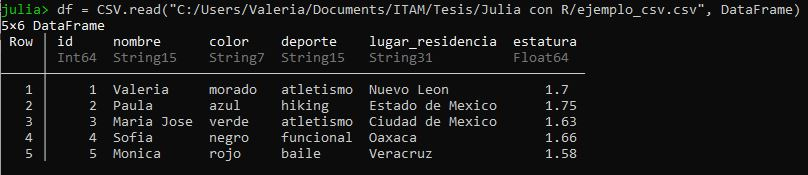
\includegraphics[scale=0.6]{Imagenes/insertar_df.JPG}
  \label{insertar_df}
\end{center}
\end{figure}

Los dataframes se pueden manejar de diferentes maneras. En este trabajo utilicé algunas de ellas, pero en caso de que tengas más dudas puedes consultar el manual oficial del paquete en \url{https://dataframes.juliadata.org/stable/}. 

\subsection{Regresiones}

\valinline{Buen link de ayuda \url{https://www.machinelearningplus.com/linear-regression-in-julia/}}

¿Cuál es el punto de tener una muestra de tamaño significativo si no sabemos analizarla? Una de las maravillas que nos regala la estadística es el uso de regresiones para intentar encontrar una explicación a los datos. Regresión es un método que permite a los investigadores resumir como predicciones o valores promedio de un resultado varían a través de variables individuales definidas como predictores. \citep{regression_other_stories} 

En pocas palabras, una regresión es una fórmula que intenta explicar como una variable depende otras. En Julia, esto se puede hacer con ayuda del paquete \texttt{GLM}, ya que facilita el cálculo de modelos lineales. Como todos los paquetes, primero hay que instalarlo usando los pasos en \ref{instalacion_paquete}. 

En este paquete la función principal se llama \texttt{glm}. En el manual oficial del paquete \cite{glm_manual} está descrita la manera en que se pueden generar modelos más avanzados. La función principal es \texttt{glm(formula, data, family, link)} donde 

\begin{itemize}
    \item \texttt{formula}: usa los nombres de las columnas del dataframe de datos para referirse a las variables predictoras
    
    \item \texttt{data}: el dataframe que contenga los predictores de las formula
    
    \item \texttt{family}: podemos elegir entre Bernoulli(), Binomial(), Gamma(), Normal(), Poisson() o NegativeBinomial() 
    
    \item \texttt{link}: se usa para especificar la función liga o \textit{link function}. La lista de posibles opciones está en el manual oficial de GLM. 
\end{itemize}


\subsubsection{Regresión lineal simple}
El modelo de regresión lineal más simple es el que tiene un solo predictor

\begin{equation*}
    \begin{aligned}
    y = a + bx + \epsilon
    \end{aligned}
\end{equation*}

Para ejemplificar este modelo de regresión use los datos de \citep{regression_other_stories}. Los datos fueron recabados por Douglas Hibbs con el objetivo de predecir las elecciones de Estados Unidos basándose solamente en el crecimiento económico. Los datos se ven de la siguiente manera: \val{Como le hago para incluir esto?}

\begin{figure}[H]
\begin{center}
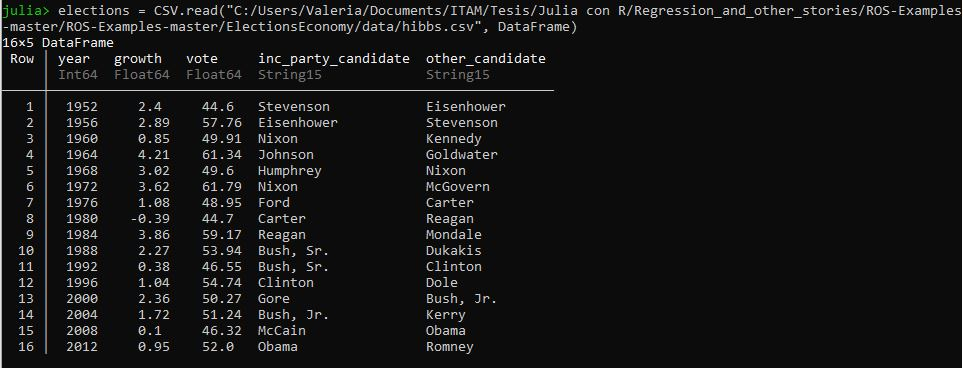
\includegraphics[scale=0.5]{Imagenes/elections_dataframe.JPG}
  \label{elections_dataframe}
\end{center}
\end{figure}

En este modelo busco que el voto sea resultado del crecimiento económico. El código para hacer esto en Julia es

\begin{minted}{julia}
	elections_lm = lm(@formula(vote ~ growth), elections)
\end{minted}

El resultado es una tabla con los coeficientes, la desviación estándar, el valor t, el valor p y el intervalo de confianza del $95 \% $ para los regresores. En este ejemplo, el resultado que da Julia es $y = 46.3 + 3.1x$ el cual coincide con los valores que da Gelman.

\subsubsection{Regresión lineal múltiple}

El caso general de la sección anterior se conoce como regresión lineal múltiple. La diferencia es que en este caso hay múltiples predictores que cumplen ciertos criterios. \cite{regression_other_stories} define este tipo de regresión como 

\begin{equation*}
    \begin{aligned}
    y_i = \beta_1 X_{i1} + \dots + \beta_k X_{ik} + \epsilon_i, \text{ para } i = 1, \dots, n
    \end{aligned}
\end{equation*}

donde los errores $\epsilon_i$ son independientes e idénticamente distribuidos de manera normal con media 0 y varianza $\sigma^2$. La representación matricial equivalente es 

\begin{equation} \label{eq_rlm}
    \begin{aligned}
        y_i = X_i \beta + \epsilon_i, \text{ para } i = 1, \dots, n
    \end{aligned}
\end{equation}

donde $X$ es una matriz de $n \times k$ con renglón $X_i$.

Para ejemplificar este tipo de modelo use un ejemplo que consta de dos predictores y la relación entre ellos. De nuevo utilicé los datos de \cite{regression_other_stories} que muestran la relación entre los resultados de exámenes de niños (\texttt{kid\_score}), el coeficiente intelectual IQ de sus madres (\texttt{mom\_iq}) y si sus madres terminaron o no la preparatoria (\texttt{mom\_hs}). 

Busco determinar si hay relación significativa entre la educación y el coeficiente de las madres con los resultados de exámenes de los niños. Por lo tanto, los predictores son las variables en relación con la madre mientras que la respuesta es el desempeño de los niños. El código en Julia se ve de la siguiente manera

\valinline{Como pongo el directorio de donde está mi base?}
\begin{minted}{julia}
    using DataFrames, GLM, CSV

    data_kid = CSV.read("C:/Users/Valeria/Documents/ITAM/Tesis/Julia con R/Regression_and_other_stories/ROS-Examples-master/ROS-Examples-master/KidIQ/data/kidiq.csv", DataFrame)

    fm = @formula(kid_score ~ mom_hs + mom_iq + mom_hs*mom_iq)

    kidscore_lm = lm(fm, data_kid)
\end{minted}

Lo cual da como resultado el modelo 

\begin{equation*}
    \begin{aligned}
        kid\_score = -11.48 + 51.26* mom\_hs + 0.97*mom\_iq \\
        -0.48*mom\_hs*mom\_iq + \epsilon
    \end{aligned}
\end{equation*}

Otro de los aspectos que hay que resaltar en este ejemplo es que para incluir la relación entre dos predictores basta usar un asterisco entre ellos al momento de definir la formula de la regresión. 

En el caso donde alguno de los regresores sea de tipo categórico la fórmula se mantiene igual pero hay que hacerle cambios a la base de datos en sí. Si Julia no reconoce estas columnas como categóricas entonces hay que cambiar su tipo en el dataframe. Abordo este problema más a fondo en el capítulo 8 \val{Checar al final que sí sea este capítulo}. Por otro lado, puedes intentar usar el paquete \texttt{CSVFiles} para leer los archivos ya que hace mejor trabajo identificando el tipo de variables. Sin embargo, este paquete todavía está en desarrollo por lo es más propenso a tener errores. 

\chapter{Ajuste de polinomios}

\section{El problema}
El problema que voy a abordar en esta sección es el mismo que abordaron \cite{laberintos} en el artículo mencionado en las referencias. Sin embargo, la diferencia es que yo utilicé Julia, R y Python  mientras que ellos compararon R, Excel, Stata, SPSS, SAS y Matlab. 

Supongamos que tenemos un conjunto de datos con solamente dos variables $x$, $y$. Buscamos ajustarlos a un polinomio de grado $k$. Es decir, buscamos ajustar los datos al modelo

\begin{equation*} 
    \begin{aligned}
    y = \sum_{j = 0}^{k} \beta_j x^j + \epsilon
    \end{aligned}
\end{equation*}

donde $j$ es el grado de la variable $x$. 

El problema consiste en encontrar los mejores coeficientes que cumplan la ecuación anterior. Una manera más compacta de ver el problema es de forma matricial 

\begin{equation}
\label{eq_matricial_pol}
    \begin{aligned}
    y = X \beta.
    \end{aligned}
\end{equation}

donde $y$ es un vector de tamaño $n$, $X$ es una matriz de tamaño $n \times (k + 1)$ y $\beta$ es un vector de tamaño $k + 1$. 


\section{Los datos}
En esta sección explicare como ajustar un conjunto de datos a un polinomio de grado $k$. Los datos que usare son proporcionados por el Instituto Nacional de Standards y Tecnología (NIST por sus siglas en inglés). Para este problema, seleccioné el conjunto llamado filip que se encuentra en \url{https://www.itl.nist.gov/div898/strd/lls/data/LINKS/DATA/Filip.dat}. Estos datos contienen 82 pares ordenados $(x_i, y_i)$. La siguiente imagen muestra las primeras 10 observaciones de los datos. 

\begin{figure}[h]
\begin{center}
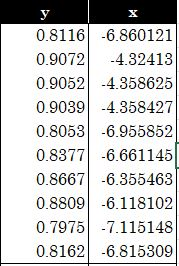
\includegraphics[scale=0.5]{Imagenes/header_filip.JPG}
  \label{header_filip}
\end{center}
\end{figure}

\valinline{no sé si agregar una gráfica rápida de los datos porque a simple vista no parecen un polinomio de grado 10}

Seleccioné este conjunto de datos porque además de proporcionar la información para el ajuste, también dan la respuesta al vector $\beta$ con alta precisión en sus dígitos. 

\section{Planteamiento del problema}

De esta forma, el vector $y$ de la ecuación \ref{eq_matricial_pol} es de tamaño 82 y corresponde a la columna $y$ del conjunto de datos.
Podríamos definir la matriz $X$ de la siguiente manera

\begin{equation*}
    \begin{aligned}
    X = 
    \begin{pmatrix}
    1 & x_{1,1} & x_{1,2} & \dots & x_{1, 10}  \\
    1 & x_{2,1} & x_{2, 2} & \dots & x_{2, 10} \\
    \vdots & \vdots & \vdots & \dots & \vdots \\
    1 & x_{81,1} & x_{81, 2} & \dots & x_{81, 10} \\
    1 & x_{82,1} & x_{82, 2} & \dots & x_{82, 10}. \\
    \end{pmatrix}
    \end{aligned}
\end{equation*} 

Representar la matriz $X$ de esta forma tiene una ventaja. Cada elemento puede ser visto como $x_{i, j}$ donde el renglón $i$ representa la observación $i$ de los datos. Por otro lado, la columna $j$ representa la potencia a la que está elevada la observación $i$. Por ejemplo, el elemento $x_{34, 5}$ es la observación 34 de los datos elevado a la 5 potencia. Sin embargo, es importante reconocer que el elemento $x_{34, 5}$ realmente está en la columna 6 de la matriz. El pequeño cambio de notación es solamente para no perder de vista la potencia de las observaciones. 


Por último, el vector $\beta$ de la ecuación \ref{eq_matricial_pol} es de dimensión 11 y es la incógnita del problema. 


En Julia, el código para cargar los datos es el siguiente: 

\begin{minted}{julia}
    using CSV, DataFrames, Polynomials
    
    filip = CSV.read("filip_data.csv", DataFrame)

    x = filip.x
    y = filip.y
    k = 10 #grado del polinomio
    n = length(x) # número de observaciones
\end{minted}

Por otro lado, para generar la matriz X creé una función que tiene como argumento una variable $k$ que representa la potencia del polinomio que quiero ajustar. 

\begin{minted}{julia}
function generar_X(k) # k es la potencia del polinomio

    n = size(filip, 1) #numero de renglones
    
    #Defino una matriz vacía
    X = Array{Float64}(undef, n, k + 1)
    # Sabemos que la primera columna siempre es un vector de unos
    X[:, 1] = ones(n)
    
    # Para el resto de la columnas,
    # elevo cada elemento a la potencia correspondiente
    for i = 1:k
        X[:, i + 1] = x.^i
    end
    return X
end
\end{minted}


\section{Métodos}

\subsection{\textit{GLM}}

Dado que el problema es ajustar una regresión lineal, el primer paquete que se viene a la mente por utilizar es \textsf{GLM}, ya que se sus siglas se traducen a 'Modelos Lineales Generalizados'.


El manual de este paquete se puede encontrar en \url{https://juliastats.org/GLM.jl/v0.11/#Methods-applied-to-fitted-models-1}. \val{No estoy segura si dejar esto o no} 

Para ajustar un modelo lineal generalizado, hay que utilizar la función \texttt{lm(formula, data)} donde 

\begin{itemize}
    \item formula: 
    Corresponde a la fórmula del ajuste con los nombres de las columnas de los datos
    \item data:
    Debe ser un dataframe con los datos por ajustar. Los datos pueden contener valores NA. 
\end{itemize}

En nuestro caso, queremos ajustar un polinomio de grado 10 a los datos guardados con el nombre de filip. Por lo tanto, el código en Julia es

\begin{minted}{julia}
    x_fit = lm(@formula(y ~ 1 + poly(x, 10)), filip)
\end{minted}

donde \texttt{poly(x, 10)} es una función con sintaxis extendida que se utiliza específicamente para regresión polinomial. Esta función viene programada en la documentación del paquete \textsf{StatsModels} en el apartado de \textsf{Extending @formula syntax} que se encuentra en la dirección \url{https://juliastats.org/StatsModels.jl/stable/internals/}. \val{No sé si mejor poner la referencia?? creo que si}



Este método no funcionó. Dado que los datos de NIST vienen con la respuesta correcta, fue claro observar que los resultados con el paquete GLM no ajustaron de manera precisa el polinomio. 

\subsection{Descomposición QR versión económica}

\begin{definition}
La factorización QR de una matriz $A$ de dimensiones $m \times n$ es el producto de una matriz $Q$ de $m \times n$ con columnas ortogonales y una matriz $R$ cuadrada y triangular superior \cite[p.~191]{garcia2017second}. 
\end{definition}

Una de las aplicaciones de la descomposición QR es dar solución a problemas de mínimos cuadrados. Por lo tanto, es el segundo método que utilizamos para obtener los valores $\beta$ de \ref{eq_matricial_pol}.

 \begin{definition}
 Una secuencia de vectores $u_1, u_2, \dots$ (finita o infinita) en un espacio de producto interno es ortonormal si 
 \begin{equation*}
     \begin{aligned}
     \langle u_i , uj \rangle = \delta_{ij} \text{ para toda $i, j$}
     \end{aligned}
 \end{equation*}
 Una secuencia ortonormal de vectores es un sistema ortonormal \cite[p.~147]{garcia2017second}.
 \end{definition}

\begin{definition}
Una base ortonormal para un espacio de producto interno finito es una base que es un sistema ortonormal \cite[p.~149]{garcia2017second}.
\end{definition}

En nuestro problema las dimensiones $m \times n$ de la matriz $X$ son $82 \times 11$. Además, $X$ tiene rango $r = 10 < n$ por lo que la matriz $R$ de la descomposición QR es singular. Como consecuencia, no se puede generar una base ortonormal de $R(X)$. Sin embargo, el proceso de factorización QR se puede modificar usando una matriz de permutación para generar una base ortonormal.


\begin{definition}
Una matriz $A$ es una matriz de permutación si exactamente una entrada en cada renglón y en calada columna es 1 y todas las otras entradas son 0 \cite[p.~183]{garcia2017second}.
\end{definition}

La idea del método QR modificado es generar una matriz de permutación $P$ tal que 

\begin{equation*}
    \begin{aligned}
    AP = QR
    \end{aligned}
\end{equation*}

donde 

\begin{equation*}
    \begin{aligned}
    R = 
    \begin{pmatrix}
    R_{11} & R_{12} \\
    0      & 0
    \end{pmatrix}
    \end{aligned}
\end{equation*}

En este caso, si tomamos $r$ como el rango de $X$ entonces $R_{11}$ es de dimensión $r \times r$ triangular superior y $Q$ es ortogonal. Las primeras $r$ columnas de $Q$ forman una base ortonormal de $R(X)$ \cite{numerical_linear_algebra}. La factorización QR con columnas pivoteadas \val{si se dice asi? le dicen version economica en el articulo pero no encuentro la traduccion} siempre existe debido al siguiente teorema.

\begin{theorem} \label{exitencia_QR_dec}
Sea $A$ una matriz de $m \times n$ con rango($A$) = $r \leq min (m, n)$. Entonces, existe una matriz de permutación $P$ de $n \times n$ y una matriz ortogonal $Q$ de dimensiones $m \times m$ tal que 
\begin{equation*}
\begin{aligned}
Q^{T}AP = 
\begin{pmatrix}
R_{11} & R_{12} \\
   0      & 0
\end{pmatrix}
\end{aligned}
\end{equation*}
donde $R_{11}$ es una matriz triangular superior de tamaño $r \times r$ con entradas en la diagonal diferentes de cero \cite[p.~532]{numerical_linear_algebra}.
\end{theorem}

\val{literal el teorema viene de Datta 2010}

Para aplicar este método en Julia, hay que usar el siguiente código

\begin{minted}{julia}
    ### Con QR Pivoted
    F = qr(X, Val(true))
    Q = F.Q
    P = F.P
    R = F.R
\end{minted}



Ya tenemos el código que calcula las matrices $P, Q, R$ de la descomposición QR con columnas pivoteadas. Para resolver nuestro problema original \ref{eq_matricial_pol} y obtener los valores de los elementos de $\beta$ hay que hacer un poco de álgebra. 



Recordemos que el problema es obtener $\beta$ de la ecuación $y = X \beta$. También, por el teorema \ref{exitencia_QR_dec}, sabemos que $X$ siempre tiene descomposición QR con columnas pivoteadas. Es decir, $XP = QR$. Por otro lado, como $P$ es matriz de permutación por lo que

\begin{equation*}
    \begin{aligned}
    \exists z \text{ tal que } Pz = \beta .
    \end{aligned}
\end{equation*}

Por lo tanto, ya tenemos una expresión para $\beta$ que podemos sustituir en la ecuación \ref{eq_matricial_pol} para obtener 
\begin{equation*}
    \begin{aligned}
    y = X (Pz) . 
    \end{aligned}
\end{equation*}

A la vez, sustituyendo en la fórmula de la descomposición QR

\begin{equation*}
    \begin{aligned}
    (XP) z = (QR) z . 
    \end{aligned}
\end{equation*}

Uniendo las dos ecuaciones anteriores, obtenemos 

\begin{equation*}
    \begin{aligned}
    y = XP z = QR z 
    \longrightarrow y = QRz
    \end{aligned}
\end{equation*}

Por lo tanto, el primer paso es resolver la ecuación 

\begin{equation*}
    \begin{aligned}
    y = QRz
    \end{aligned}
\end{equation*}

Para finalmente obtener $\beta$ calculando 
\begin{equation*}
    \begin{aligned}
    \beta = Pz
    \end{aligned}
\end{equation*}

En Julia, esto se programa de la siguiente manera
\begin{minted}{julia}
    # 1. Resolver QRz = y
    z = Q*R \ y
    # 2. Resuelvo beta = Pz
    x_QR = P*z
\end{minted}


Este método tampoco funcionó. Podemos empezar a consider que los datos son tan sensibles que la propagación del error es tal que no permite un buen ajuste del polinomio. Intentaremos con otros dos métodos.

\subsection{Descomposición de valores singulares}

La tercer manera en la que intenté resolver este problema fue usando la descomposición de valores singulares para obtener la matriz pseudoinversa de Moore-Penrose. 

\begin{definition}
Sea $A$ una matriz de $m \times n$ y sea $q = min \{m, n \}$. Si el rango de $A = r \geq 1$, sean $\sigma_1 \geq \sigma_2 \geq \dots \geq \sigma_r > 0$ los eigenvalores positivos en orden decreciente de $(A^{*}A)^{1/2}$. Los valores singulares de $A$ son
\begin{equation*}
    \begin{aligned}
    \sigma_1, \sigma_2, \dots, \sigma_r \text{ y } \sigma_{r+1} = \sigma_{r+2} = \dots = \sigma_q = 0.
    \end{aligned}
\end{equation*}
Si A = 0, entonces los valores singulares de A son $\sigma_1 = \sigma_2 = \dots = \sigma_q = 0$. 
Los valores singulares de $A \in M_{n}$ son los eigenvalores de $(A^{*}A)^{1/2}$ que son los mismos eignevalores de $(AA^{*})^{1/2}$
\cite[p.~420]{garcia2017second}
\end{definition}

Los valores singulares tienen muchas apliciones. Sin embargo, para resolver ecuaciones lineales son usados para obtener la descomposición de valores singulares (DVS). 


\begin{theorem}
Sea $A \in M_{m \times n} (F)$ diferente de cero y sea $r =   rango(A)$. Sean $\sigma_1 \geq \sigma_2 \geq \dots \geq \sigma_r > 0$ los valores singulares positivos de A y definamos

\begin{equation*}
    \begin{aligned}
    \Sigma_r = 
    \begin{pmatrix}
    \sigma_1 & & 0 \\
     & \ddots & & \\
     0 & & \sigma_r
    \end{pmatrix}
    \in M_{r}(R).
    \end{aligned}
\end{equation*}
Entonces, existen matrices unitarias $U \in M_{m}(F)$ y $V \in M_{n}(F)$ tales que 
\begin{equation} \label{decomposicion}
    \begin{aligned}
    A = U \Sigma V^{*}
    \end{aligned}
\end{equation}
donde
\begin{equation*}
    \begin{aligned}
    \Sigma = 
    \begin{pmatrix}
    \Sigma_r & 0_{r \times (n-r)} \\
    0_{(m-r) \times r} & 0_{(m-r) \times (n-r)}
    \end{pmatrix}
    \in M_{m \times n}(R)
    \end{aligned}
\end{equation*}
 tiene las mismas dimensiones que A. Si m = n, entonces $U, V \in M_{n}(F)$ y $\Sigma = \Sigma_r \oplus 0_{n-r}$.
 \cite[p.~421]{garcia2017second}
\end{theorem}

La ecuación \ref{decomposicion} con las características del teorema anterior lleva por nombre descomposición en valores singulares (DVS). 


Es importante observar que las matrices $U$ y $V$ son matrices unitarias. Es decir, 

\begin{equation*}
    \begin{aligned}
    U U^{*} u = u, \text{ } \forall u \in Col (U)
    \end{aligned}
\end{equation*}

\begin{equation*}
    \begin{aligned}
    V V^{*} v = v, \text{ } \forall v \in Col (V)
    \end{aligned}
\end{equation*}

\subsubsection{Pseudoinversa de Moore-Penrose}

Ya que conocemos la descomposición de valores singulares, podemos avanzar y definir la descomposición de valores singulares para la pseudoinversa de Moore Penrose. 

\begin{theorem}
Sea $A$ una matriz de $m \times n$ de rango $r$ con una descomposición en valores singulares de $A = U \Sigma V^{*}$ y valores singulares diferentes de cero $\sigma_1 \geq \sigma_2 \geq \dots \geq \sigma_r$. Sea $\Sigma^{\dagger}$ una matriz de $n \times m$ definida como
\begin{equation*}
    \begin{aligned}
   \Sigma^{\dagger}_{ij} =
   \begin{cases}
   \dfrac{1}{\sigma_i} \text{ si } i = j \leq r\\
   0 \text{ en otro caso.}
   \end{cases}
    \end{aligned}
\end{equation*}
Entonces $A^{\dagger} = V \Sigma^{\dagger} U ^{*}$ y esta es la descomposición de valores singulares de $A^{\dagger}$. 
\cite[p.~414]{friedberglinearalgebra}
\end{theorem}

Podemos ver que en realidad lo único que cambia al calcular la pseudoinversa es la matriz $\Sigma$. Sin embargo, esta nueva matriz $A^{\dagger}$ tiene propiedades interesantes. 

\begin{itemize}
    \item $(A^{T}A)^{\dagger} A^{T} = A^{\dagger}$
    \item $(AA^{T})^{\dagger} A = (A^{\dagger})^{T}$
    \item $(A^{T}A)^{\dagger}(A^{T}A) = A^{\dagger}A = VV^{T}$
\end{itemize}


Recordando que buscamos obtener $\beta$ que satisfaga la ecuación \ref{eq_matricial_pol} podemos ver que el sistema lineal está sobredeterminado. Esto se puede verificar por las dimensiones de la matriz $X_{n \times m} = X_{82 \times 11}$. Como $m < n$, sabemos que hay más ecuaciones que variables desconocidas. 


\valinline{Como sabemos que y esta en el espacio de columnas de V?}
De la ecuación \ref{eq_matricial_pol} podemos multiplicar por $X^{T}$ para obtener
\begin{equation}
\label{transformacion_eq_base}
    \begin{aligned}
    X^{T}X \beta = X^{T} y, \text{ } y \in Col(V).
    \end{aligned}
\end{equation}

La ecuación \ref{transformacion_eq_base} siempre da un sistema determinado (balanceado) \cite{worldScientificNews}. Ahora bien, multiplicando \ref{transformacion_eq_base} por $(X^{T}X)^{\dagger}$ y usando las propiedades de la matriz pseudo inversa podemos obtener 


\begin{equation*}
    \begin{aligned}
    (X^{T}X)^{\dagger} X^{T}X \beta = (X^{T}X)^{\dagger} X^{T} y \\
    \iff X^{\dagger} X \beta = X^{\dagger} y \\
    \iff V V^{T} \beta = X^{\dagger} y \\
    \beta = X^{\dagger} y 
    \end{aligned}
\end{equation*}. 

Por lo tanto, la pseudo inversa de Moore Penrose da la solución de mínimos cuadrados de \ref{eq_matricial_pol} \cite{worldScientificNews}


En Julia, este método se puede programar de la siguiente manera:

\begin{minted}{julia}
    # # # Inversa de Moore Penrose
    N = pinv(X)
    aux = ones(k + 1)
    x_MP = N*y 
\end{minted}

Este método tampoco funcionó. Por lo tanto, investigue más a fondo los paquetes de Julia hasta encontrar el paquete \textit{Polynomials}. 

\subsection{\textit{Polynomials}}
\textit{Polynomials} es un paquete que proporciona aritmética básica, integración, diferenciación, evaluación y hallar raíces para polinomios univariados \cite{poly_manual}. Para poder usar el paquete primero hay que descargarlo usando el código \ref{instalacion_paquete}. 


El paquete \textit{Polynomials} tiene su propia función \texttt{fit} que toma tres variables como entrada. Las primeras dos entradas son las correspondientes a $x$ y $y$ de los datos a utilizar (en este caso, los datos filip). La tercera entrada corresponde al grado que buscamos que sea el polinomio (en este caso, grado 10). 

A diferencia de los otros método utilizados para este problema, la función \texttt{fit} usa el metódo Gauss-Newton para resolver sistemas de ecuaciones no lineales. Sin embargo, en este caso tenemos un problema lineal. Esta fue la primera razón por la que este paquete no fue mi primera opción para resolver el problema. 
\valinline{No sé si tengo que explicar este método}


La segunda razón es que a diferencia de la función \texttt{lm} del paquete \textit{GLM}, la función \texttt{fit} solamente aporta los coeficientes del ajuste del polinomio. Es decir, no da como resultado el error estandar, ni el valor p de la estimación. Sin embargo, tengo que agregarlo a esta sección de la tesis, ya que es el único método que funcionó. 


El código en Julia se ve de la siguiente manera:

\begin{minted}{julia}
using Polynomials 
x_pol = Polynomials.fit(x, y, 10)
\end{minted}


Este método fue el único de los cuatro que funcionó para el polinomio de grado 10. La desventaja de este método es que la función solamente arroja los coeficientes $\beta$. Si quisieramos ampliar el análisis y observar, por ejemplo, el valor p de algún regresor tendríamos que buscar otra manera de obtenerlo. 


\section{Evaluación de los métodos}
Una cuestión válida es preguntarse si tal vez lo que está mal es la implementación de los algoritmos y, debido a esto, no dan la respuesta correcta. Por tanto, para probar que los métodos estén programados de la manera correcta los somentí a una serie de pruebas.


La primera prueba consiste en que, usando los datos filip, cada método ajustaba un polinomio de grado $k$ de $k = 1, 2, \dots, 10$. Al final, para cada polinomio de grado $k$ tenía cuatro resultados de ajuste (uno por cada método). 

La segunda prueba consiste en comparar los resultados con R. De manera análoga a Julia, en R también use los datos filip para ajustar un polinomio de grado $k$ de $k = 1, 2, \dots, 10$. Para esto, use la función \texttt{lm(formula, data)} donde los datos siempre son los mismos y la fórmula depende del grado del polinomio. Es importante mencionar que este problema ya ha sido abordado por otros usuarios y resuelto por Brian Ripley. Ripley es un matemático británico que ha escrito muchos libros sobre programación y ha ganado muchos premios por sus aportaciones a la estadística. Sin duda lo más relevante en este caso es que es uno de los contribuidores principales en el desarrollo de \textsf{R}. El código que utilicé para resolver este problema es el mismo que Ripley hizo público. 


La tercera prueba fue medir el tiempo que tomaba a R ejecutar la función \texttt{lm} con los parametros especificados. El código es el siguiente: 

\begin{minted} {R}
# Para polinomio de grado = 1
start <- Sys.time()
lm_1 <- lm(y ~ x, data = data, x = TRUE)
end <- Sys.time()

`resultados_grado_ 1`$R <- lm_1$coefficients
row.names(`resultados_grado_ 1`) <- c("b0", "b1")
X_1 <- lm_1$x

time_vec <- c(end - start)

# Para polinomios de grado > 1

for (i in 2:10){
  #Hacemos el modelo
  model <- paste("y ~ x", paste("+ I(x^", 2:i, ")", sep='', collapse=''))
  
  # Lo convertimos en formula
  form <- formula(model)
  
  #Ejecutamos el modelo
  start <- Sys.time()
  lm.plus <- lm(form, data = data, x = TRUE)
  end <- Sys.time()
  time <- end - start
  time_vec <- c(time_vec, time)
  
  # Guardo el df correspondiente a un auxiliar
  resultados_aux <- get(paste("resultados_grado_", i))
  # para unirle los coeficientes
  resultados_aux$R <- lm.plus$coefficients
  
  nombres <- c("b0")
  # Para el nombre de los renglones
  for (k in 1:i){
    nombres <- c(nombres, paste0("b", k))
  }
  row.names(resultados_aux) <- nombres
  
  #Finalmente, hago el df final
  assign(paste("resultados_grado_", i), resultados_aux)
  
  assign(paste("X_", i), lm.plus$x)
 
\end{minted}

No voy a mostrar todas las tablas con los resultados ya que son muchas. Me voy a limitar a las tablas que considero tienen los resultados más relevantes. Para el polinomio de grado 1, todos los métodos obtienen los mismos resultados. 

\begin{figure}[h]
\begin{center}
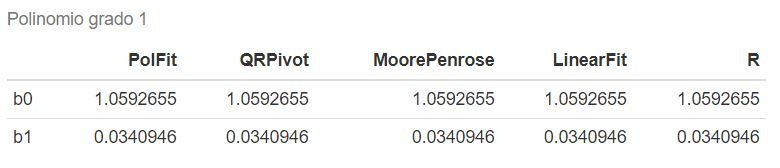
\includegraphics[scale=0.5]{Imagenes/tabla_pol_1.JPG}
\end{center}
\end{figure}

Todos los métodos funcionan bien calculando el ajuste hasta llegar al polinomio de grado 5. Cuando calculamos el polinomio de grado 6, el método \texttt{fit} del paquete \texttt{GLM} llamado \texttt{LinearFit} comienza a fallar. 

\begin{figure}[h]
\begin{center}
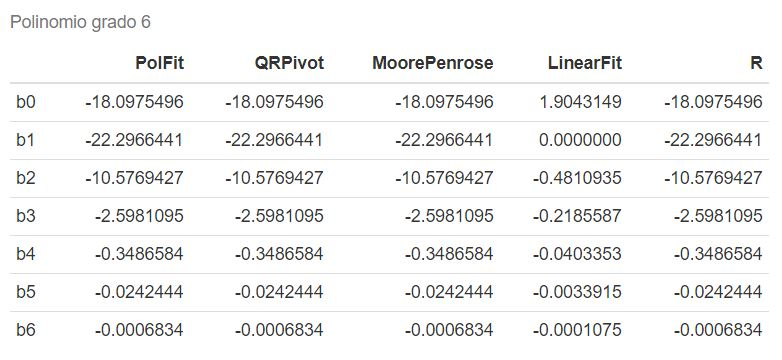
\includegraphics[scale=0.5]{Imagenes/tabla_pol_6.JPG}
\end{center}
\end{figure}

A partir del polinomio de grado 6, \texttt{LinearFit} comienza a fallar y comienza a dar resultados muy érroneos. Todos los métodos arrojan resultados correctos hasta que llegamos al polinomio de grado 10. 

\begin{figure}[h]
\begin{center}
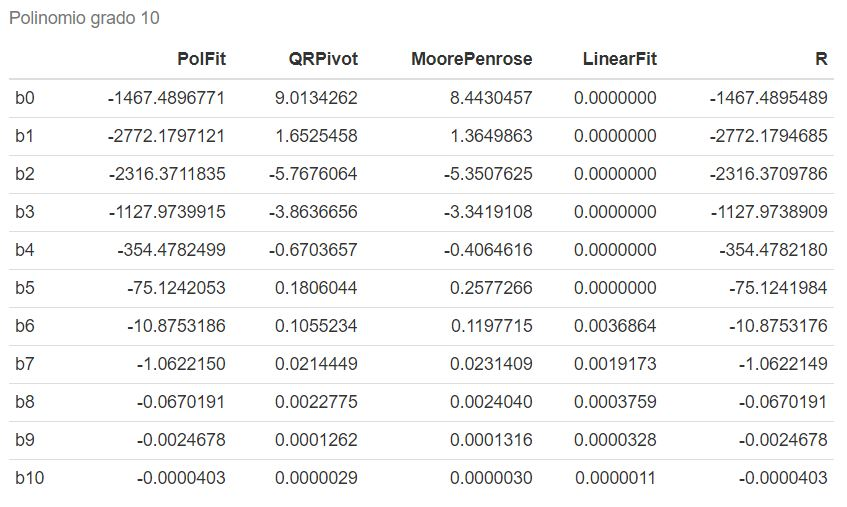
\includegraphics[scale=0.5]{Imagenes/tabla_pol_10.JPG}
\end{center}
\end{figure}

Finalmente, podemos ver la tabla de tiempos que le tomo a cada método. Las columnas representan los métodos usados mientras que los renglones el grado de polinomio que se ajustó. 

\begin{figure}[h]
\begin{center}
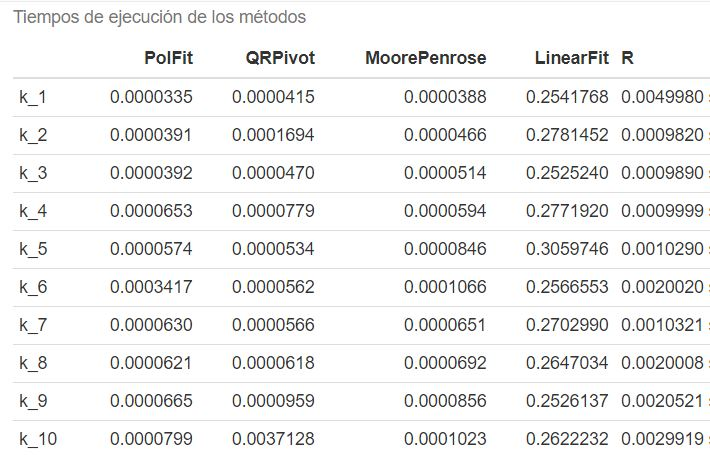
\includegraphics[scale=0.5]{Imagenes/table_tiempos.JPG}
\end{center}
\end{figure}

\valinline{Las tablas están por donde quieren, mejor copio los resultados?}



\section{Eigenvalores y valores singulares}
\valinline{No estoy segura de que poner dado que no sale la igualdad basica entre eigenvalores y valores singulares}

\section{Número de condición y precisión de la solución}

\begin{definition}
El número $\parallel A \parallel  \parallel A^{-1} \parallel$ se llama el número de condición de $A$ y se denota $Cond(A)$ \cite[p.~62]{numerical_linear_algebra}. 
\end{definition}

Como vimos en la sección de Evaluación de los métodos, los métodos sí están bien programados. Dejando de lado las funciones programadas por default en Julia, el método de factorización QR y descomposición de valores singulares arrojaron buenos resultados hasta los polinomios de grado 9. Esto nos puede llevar a pensar que en realidad, los datos en sí son muy susceptibles a cambios. Es decir, cualquier cambio en la matriz $X$ o en el vector $y$ resultara en un ajuste de los coeficientes $\beta$ poco preciso. Esta cualidad también se conoce como que los datos tienen impurezas. El caso contrario, donde los métodos dan resultados precisos se conoce a los datos como exactos \cite{numerical_linear_algebra}.


En general, para nuestro problema \ref{eq_matricial_pol} tenemos tres casos: 
\begin{itemize}
    \item El vector $y$ tiene impurezas mientras que la matriz $X$ es exacta. 
    \item La matriz $X$ tiene impurezas mientras que el vector $y$ es exacto
    \item Ambos, el vector $y$ y la matriz $X$ tiene impurezas. 
\end{itemize}

En nuestro caso, nos vamos a enfocar en el tercer caso ya que no tenemos razón para pensar que solamente una columna de los datos originales tiene impurezas mientras que la otra no. 


\begin{theorem} \label{teo:perturbaciones}
Supongamos que queremos resolver el sistema $Ax = b$. Supongamos que $A$ es no singular, $b \neq 0$, y $\parallel \Delta A \parallel < \dfrac{1}{\parallel A^{-1} \parallel}$. Entonces
\begin{equation*}
    \begin{aligned}
    \dfrac{\parallel \delta x \parallel}{\parallel x \parallel} \leq (\dfrac{Cond(A)}{1 - Cond(A) \dfrac{\parallel \Delta A \parallel}{\parallel A \parallel}}) (\dfrac{\parallel \Delta A \parallel}{\parallel A \parallel} + \dfrac{\parallel \delta b \parallel}{\parallel b \parallel})
    \end{aligned}
\end{equation*} \cite[p.~65]{numerical_linear_algebra}
\end{theorem}

El teorema anterior nos está diciendo que los cambios en la solución $x$ son menor o iguales a una constante determinada por el número de condición multiplicada por la suma de las pertubaciones de $A$ y las pertubaciones de $b$. Además, el teorema nos dice que aunque las perturbaciones de $A$ y $b$ son pequeñas, puede haber un cambio grande en la solución si el número de condición es grande. Por lo tanto, $Cond(A)$ juega un papel crucial en la sensibilidad de la solución \cite{numerical_linear_algebra}. 


El número de condición tiene varias propiedades pero en la que nos queremos centrar es en la siguiente: 

\begin{equation} \label{formula:num_cond}
    \begin{aligned}
    Cond(A) = \dfrac{\sigma_{max}}{\sigma_{min}}
    \end{aligned}
\end{equation}

donde $\sigma_{max}$ y $\sigma_{min}$ son, respectivamente, el valor singular más grande y más pequeño de $A$. 

Antes de calcular el número de condición de nuestra matriz $X$ de \ref{eq_matricial_pol}, vamos a ver una última definición. 

\begin{definition} \label{def:condicionamiento}
El sistema $Ax = b$ está mal condicionado si el $Cond(A)$ es grande (por ejemplo, $10^{5}, 10^{8}, 10^{10}, etc)$. En otro caso, está bien condicionado \cite[p.~68]{numerical_linear_algebra}.
\end{definition}

Ahora vamos a calcular el número de condición. Este calculo lo hice en Julia y en R usando ambos, la función que ya viene programada en cada lenguaje y usando la fórmula \ref{formula:num_cond}. En Julia, el código es 

\begin{minted}{julia}
# Con función de Julia
numcond_1 = cond(X_10)

# Usando propiedad de valores singulares
sing_values = svd(X_10).S
sing_values = sort(sing_values)
numcond_2 = sing_values[length(sing_values)] / sing_values[1]
\end{minted}

Los resultados son $numcond_1 = 1.7679692504686805e15$ y $numcond_2 = 1.7679692504686795e15$. Por otro lado, en R el código es 

\begin{minted}{R}
# con función de R
numcond_R1 <- cond(X)

# Usando propiedad de valores singulares
S.svd <- svd(X)
S.d <- S.svd$d
S.d <- sort(S.d, decreasing = TRUE)
numcond_R2 <- S.d[1] / S.d[length(S.d)]
\end{minted}

Los resultados son $numcond_{R1} = numcond_{R2} = 1.767962e{15}$. En conclusión, en ambos lenguajes cualquier método confirma que el número de condición de la matriz $X$ de \ref{eq_matricial_pol} es bastante grande por lo que por \ref{def:condicionamiento} sabemos que nuestro problema está mal condicionado. \valinline{Tengo duda, entonces alguien me podría decir que para que los uso}








\chapter{R}
Porque juntar Julia con R. Usar documentación oficial: https://cran.r-project.org/web/packages/JuliaCall/JuliaCall.pdf. También en esta sección incluir muchos ejemplos prácticos 

\section{Paquete JuliaCall}
Como instalarlo en R 

\subsection{install\_julia}

\subsection{julia\_setup}
De este no estoy segura, tengo que checar en las cosas de Rodrigo

\subsection{Núcleos y threads}

\subsection{JuliaObject}

\subsection{julia\_assign}

\subsection{julia\_eval}

\subsection{julia\_package}

\section{Ejemplo}
\chapter{Computadoras virtuales}

\section{Amazon}
Como hacer una computadora virtual en Amazon que me haga todo esto. El tutorial oficial de como instalarlo en Amazon está aquí: \url{https://d1.awsstatic.com/whitepapers/julia-on-sagemaker.pdf?did=wp_card&trk=wp_card}

\section{Docker}
También se podría usar Docker pero te quita espacio en tu computadora y puede crashear como la mía. Para Windows como que no está muy bonito el asunto pero al parecer para Linux sí. También podría ser opción idk 


%----------------------------------------------------------------------------------------
%	APÉNDICES
%----------------------------------------------------------------------------------------

\begin{appendix}

\chapter{Extras}
No se olviden cambiar toda la información. Los quiero un chingo

\end{appendix}

%----------------------------------------------------------------------------------------
%	BIBLIOGRAFÍA
%----------------------------------------------------------------------------------------

\bibliography{referencias}
\bibliographystyle{chicago}

\newpage
\thispagestyle{empty}
\begin{center}
\begin{minipage}{.6\linewidth}
\begin{center}
\vspace{3cm}
\begin{small}
\textit{\thetitle}, escrito por \theauthor , se terminó de imprimir de madrugada,\\ con mucha cafeína en las venas\\ y ojeras en la cara. %Le ponen el nombre del lugar donde la manden a imprimir, la ciudad y el año
\end{small}
\end{center}
\end{minipage}
\end{center}

% Si lo prefieren, avisen a su taller que esta página ya la incluyeron ustedes para que no les impriman las que ellos usan. Lo recomiendo ampliamente

%%%%%%%%%%%%%%%%%%%%%%%%%%%%%%%%%%%%%%%%%%%%%%%%%%%%%%%%%%%%%%%%%%%%%%%%%%%%%%%%%%%%%%%

\end{document}